\documentclass[letterpaper]{article}

\usepackage{graphics}
\usepackage{graphicx}
\usepackage{amsmath}

\title{Notes on a nonaxisymmetric global stability code in axially periodic
cylindrical geometry}
\author{Austin Roach}


\begin{document}
\maketitle{}

\section{Introduction}

Recently, nonaxisymmetric MHD modes have been observed in the
Princeton MRI experiment$^1$.  Previous computational work in support
of the experiment has been almost exclusively axisymmetric.  This work
will follow a similar approach to Goodman and Ji's examination of
unstable axisymmetric global linear modes in a cylindrical system$^2$,
but will extend the analysis to allow examination of nonaxisymmetric
eigenmodes, eigenmodes with non-ideal Couette rotation profiles, and
damped eigenmodes.

\section{Linearized equations}

We start with the equations of incompressible, nonideal MHD in cgs units:

\begin{align}
&\dot{\vec{B}} + \vec{v}\cdot\nabla\vec{B} - \vec{B}\cdot\nabla\vec{v}
 = \eta\nabla^2 \vec{B}
\\
&\dot{\vec{v}}+\vec{v}\cdot\nabla\vec{v}+\frac{1}{\rho}\nabla{P}
 - \frac{\vec{B}\cdot\nabla\vec{B}}{4\pi\rho}=\nu\nabla^2\vec{v}
\\
&\nabla\cdot\vec{B}=0
\\
&\nabla\cdot\vec{v}=0
\end{align}

Here $P$ is defined as the sum of the hydrodynamic and magnetic
pressures, $P=p+\vec{B}^2/8\pi$.We assume a background state with
zeroth-order $\vec{B}=B_0 \hat{z}$ and $\vec{
  v}=r\Omega(r)\hat{\theta}$.  First order quantities will be denoted
by a $\delta$.

We will define two radial derivative operators, $\partial_r \equiv
\frac{\partial}{\partial r}$ and $\partial_{r}^\dagger \equiv
\frac{\partial}{\partial r}+\frac{1}{r}$.  The combination
$\partial_r \partial_r^\dagger = \frac{\partial^2}{\partial
  r^2}-\frac{1}{r^2}+\frac{1}{r}\partial_r$.

\subsection{Radial induction equation}

The radial component of the induction equation is
\begin{align}
\dot{B_r} + v_r \partial_r B_r + \frac{v_\theta}{r}\partial_\theta B_r
 + v_z \partial_z B_r - B_r \partial_r v_r
 -\frac{B_\theta}{r}\partial_\theta v_r - B_z \partial_z v_r
\nonumber \\
= \eta\left(\nabla^2 B_r -\frac{2}{r^2}\partial_\theta B_\theta
 - \frac{1}{r^2}B_r\right)
\end{align}
After linearization, keeping only 1st-order quantities, this becomes
\begin{equation}
\delta \dot{B_r} + \Omega \partial_\theta \delta B_r
 - B_0 \partial_z \delta v_r = \eta\left[\left(\partial_r \partial_r^\dagger
 + \frac{1}{r^2}\partial_\theta^2 + \partial_z^2\right)\delta B_r
 - \frac{2}{r^2}\partial_\theta \delta B_\theta\right]
\end{equation}

\subsection{Azimuthal induction equation}
The azimuthal component of the induction equation is
\begin{align}
\dot{B_\theta}+v_r \partial_r B_\theta
 + \frac{v_\theta}{r}\partial_\theta B_\theta + v_z \partial_z B_\theta
 + \frac{v_\theta}{r}B_r - B_r\partial_r v_\theta
 - \frac{1}{r}B_\theta \partial_\theta v_\theta
\nonumber \\
- B_z \partial_z v_\theta - \frac{v_r}{r}B_\theta
 = \eta\left(\nabla^2 B_\theta + \frac{2}{r^2}\partial_\theta B_r
 - \frac{1}{r^2}B_\theta \right)
\end{align}
After linearization, this becomes
\begin{align}
\delta \dot{B_\theta} + \Omega \partial_\theta \delta B_\theta
 - B_0 \partial_z \delta v_\theta - \delta B_r r \partial_r \Omega
 = \eta\left[\left(\partial_r \partial_r^\dagger
 + \frac{1}{r^2}\partial_\theta^2 + \partial_z^2\right)\delta B_\theta
 + \frac{2}{r^2}\partial_\theta \delta B_r\right]
\end{align}

\subsection{Axial induction equation}
The axial component of the induction equation is
\begin{align}
\dot{B_z} + v_r \partial_r B_z + \frac{v_\theta}{r}\partial_\theta B_z
 + v_z \partial_z B_z - B_r \partial_r v_z
 - \frac{1}{r}B_\theta \partial_\theta v_z - B_z \partial_z v_z
\nonumber \\
=\eta\left[\frac{1}{r}\partial_r + \partial_r^2
 + \frac{1}{r^2}\partial_\theta^2 + \partial_z^2\right]B_z
\end{align}
After linearization this becomes
\begin{align}
\delta\dot{B_z} + \Omega\partial_\theta \delta B_z - B_0\partial_z \delta v_z
 = \eta\left[\partial_r^\dagger \partial_r + \frac{1}{r^2}\partial_\theta^2
 + \partial_z^2\right]\delta B_z
\end{align}

\subsection{Radial momentum equation}

The radial component of the Euler equation is
\begin{align}
\dot{v_r} + v_r \partial_r v_r + \frac{v_\theta}{r}\partial_\theta v_r
 + v_z \partial_z v_r - \frac{v_\theta^2}{r}+\frac{1}{\rho}\partial_r P 
\nonumber \\
- \frac{1}{4\pi\rho}\left(B_r \partial_r B_r
 + \frac{B_\theta}{r}\partial_\theta B_r + B_z \partial_z B_r
 - \frac{B_\theta^2}{r}\right)
\nonumber \\
= \nu\left(\nabla^2 v_r -\frac{2}{r^2}\partial_\theta v_\theta
 - \frac{1}{r^2}v_r\right)
\end{align}
After linearization this becomes
\begin{align}
\delta\dot{v_r} + \Omega \partial_\theta \delta v_r - 2\Omega\delta v_\theta
 + \partial_r \frac{\delta P}{\rho}
 - \frac{B_0}{4\pi\rho}\partial_z \delta B_r
\nonumber \\
= \nu \left[\left(\partial_r \partial_r^\dagger
 + \frac{1}{r^2}\partial_\theta^2 + \partial_z^2\right)\delta v_r
 - \frac{2}{r^2}\partial_\theta \delta v_\theta\right]
\end{align}

\subsection{Azimuthal momentum equation}
The azimuthal component of the Euler equation is
\begin{align}
\dot{v_\theta} + v_r \partial_r v_\theta
 + \frac{v_\theta}{r}\partial_\theta v_\theta + v_z \partial_z v_\theta
 + \frac{v_\theta v_r}{r} + \frac{1}{\rho}\frac{1}{r}\partial_\theta P 
\nonumber \\
-\frac{1}{4\pi\rho}\left[B_r\partial_r B_\theta
 + \frac{B_\theta}{r}\partial_\theta B_\theta + B_z \partial_z B_\theta
 + \frac{B_\theta B_r}{r}\right]
\nonumber \\
= \nu\left(\nabla^2 v_\theta + \frac{2}{r^2}\partial_\theta v_r
 - \frac{1}{r^2}v_\theta \right)
\end{align}
After linearization this becomes
\begin{align}
\delta \dot{v_\theta} + \delta v_r \partial_r^\dagger(r\Omega)
 + \Omega \partial_\theta \delta v_\theta
 + \frac{1}{r}\partial_\theta \frac{\delta P}{\rho}
 - \frac{B_0}{4\pi\rho} \partial_z \delta B_\theta
\nonumber \\
= \nu\left[\left(\partial_r \partial_r^\dagger
 + \frac{1}{r^2}\partial_\theta^2 + \partial_z^2\right)\delta v_\theta
 + \frac{2}{r^2}\partial_\theta \delta v_r \right]
\end{align}

\subsection{Axial momentum equation}
The axial component of the Euler equation is
\begin{align}
\dot{v_z} + v_r \partial_r v_z + \frac{v_\theta}{r}\partial_\theta v_z
 + v_z \partial_z v_z + \frac{1}{\rho}\partial_z P
\nonumber \\
-\frac{1}{4\pi\rho}\left[B_r\partial_r B_z
 + \frac{B_\theta}{r}\partial_\theta B_z + B_z \partial_z B_z \right]
\nonumber \\
=\nu\left[\frac{1}{r}\partial_r + \partial_r^2
 + \frac{1}{r^2}\partial_\theta^2 + \partial_z^2\right]v_z
\end{align}
After linearization this becomes
\begin{align}
\delta\dot{v_z} + \Omega \partial_\theta \delta v_z
 + \partial_z \frac{\delta P}{\rho} 
 - \frac{B_0}{4\pi\rho} \partial_z \delta B_z
 = \nu\left[\partial_r^\dagger \partial_r + \frac{1}{r^2}\partial_\theta^2
 + \partial_z^2\right]\delta v_z
\end{align}

\subsection{Equations of constraint}

The equation of incompressibility, $\nabla\cdot\vec{v}=0$ is
\begin{align}
\partial_r^\dagger \delta v_r + \frac{1}{r}\partial_\theta \delta v_\theta
 + \partial_z \delta v_z = 0
\end{align}
and $\nabla\cdot\vec{B}=0$ is
\begin{align}
\partial_r^\dagger \delta B_r + \frac{1}{r}\partial_\theta \delta B_\theta
 + \partial_z \delta B_z = 0
\end{align}

\section{Forms of perturbations}

These linearized equations will be evaluated to find modes with an
arbitrary radial dependence that grow exponentially with a growth rate
$\gamma$, and vary periodically in $\hat{\theta}$ and $\hat{z}$ with
mode numbers $m$ and $k$, respectively\footnote{The linearized quantities
have a time behavior that goes as $e^{\gamma t}$. Comparing to the
time behavior for the form of a wave traveling in the positive
direction, $e^{i(\vec{k} \cdot \vec{x} - \omega t)}$, we see that
$\mathrm{Re}\{\gamma\} = \mathrm{Im}\{\omega\}$, and
$\mathrm{Im}\{\gamma\} = -\mathrm{Re}\{\omega\}$. So the growth rate
of the mode is given by $\mathrm{Re}\{\gamma\}$, and the oscillation
frequency is given by $-\mathrm{Im}\{\gamma\}$.}.
The equations suggest the phase relation between the various
components in $\hat{z}$, leading to the following forms for the
first-order perturbations:

\begin{align}
&\delta B_r / \sqrt{4\pi\rho} = \operatorname{Re}\{\beta_r (r)
 e^{\gamma t + im\theta}\cos{kz}\},\quad
&\delta v_r = \operatorname{Re}\{\phi_r (r)
 e^{\gamma t + im\theta} \sin{kz}\}
\nonumber \\
&\delta B_\theta / \sqrt{4\pi\rho} = \operatorname{Re}\{\beta_\theta (r)
 e^{\gamma t + im\theta} \cos{kz}\},\quad
&\delta v_\theta = \operatorname{Re}\{\phi_\theta (r)
 e^{\gamma t + im\theta} \sin{kz}\}
\nonumber \\
&\delta B_z / \sqrt{4\pi\rho} = \operatorname{Re}\{\beta_z (r)
 e^{\gamma t + im\theta} \sin{kz}\},\quad
&\delta v_z = \operatorname{Re}\{\phi_z (r) e^{\gamma t+im\theta}\cos{kz}\}
\nonumber \\
&\delta P/ \rho = \operatorname{Re}\{\Pi (r)
 e^{\gamma t + im\theta} \sin{kz}\}&
\end{align}

The quantities $\beta$, $\phi$, and $\Pi$ are complex, holding
information about both the magnitude and phase of these components as
functions of $r$. Following the convention common in harmonic
analysis, the real parts of the perturbed forms are evaluated to find
physically meaningful quantities. Because the equations are linear, we
are justified in dropping the `$\mathrm{Re}$' when rewriting the
equations in terms of these perturbed quantities. Note that we have
made use of the Alfv\'{e}n speed, $v_A = B_0/\sqrt{4\pi\rho}$.

\begin{equation}\label{eqn:globalcode:rind_p}
\gamma \beta_r + im\Omega\beta_r - kv_A\phi_r
 = \eta\left[\left(\partial_r \partial_r^\dagger
 - \frac{m^2}{r^2} - k^2\right)\beta_r - \frac{2im}{r^2}\beta_\theta\right]
\end{equation}
\begin{equation}\label{eqn:globalcode:tind_p}
\gamma \beta_\theta + im\Omega\beta_\theta - kv_A \phi_\theta
 - r(\partial_r \Omega)\beta_r
 = \eta\left[\left(\partial_r \partial_r^\dagger
 - \frac{m^2}{r^2} - k^2\right)\beta_\theta + \frac{2im}{r^2}\beta_r\right]
\end{equation}
\begin{equation}\label{eqn:globalcode:zind_p}
\gamma \beta_z + im\Omega\beta_z + kv_A \phi_z
 = \eta\left[\left(\partial_r^\dagger \partial_r
 -\frac{m^2}{r^2} - k^2\right)\beta_z\right]
\end{equation}
\begin{equation}\label{eqn:globalcode:reul_p}
\gamma \phi_r + im\Omega\phi_r - 2\Omega\phi_\theta + \partial_r \Pi
 + kv_A\beta_r = \nu\left[\left(\partial_r \partial_r^\dagger
 - \frac{m^2}{r^2} - k^2\right)\phi_r - \frac{2im}{r^2}\phi_\theta\right]
\end{equation}
\begin{equation}\label{eqn:globalcode:teul_p}
\gamma \phi_\theta + im\Omega\phi_\theta + \phi_r \partial_r^\dagger(r\Omega)
 + \frac{im}{r}\Pi + kv_A \beta_\theta
 = \nu\left[\left(\partial_r \partial_r^\dagger - \frac{m^2}{r^2} 
 - k^2\right)\phi_\theta + \frac{2im}{r^2}\phi_r\right]
\end{equation}
\begin{equation}\label{eqn:globalcode:zeul_p}
\gamma \phi_z + im\Omega{\phi_z} + k\Pi - kv_A \beta_z
 = \nu\left[\left(\partial_r^\dagger \partial_r 
 - \frac{m^2}{r^2} - k^2\right)\phi_z\right]
\end{equation}
\begin{equation}\label{eqn:globalcode:inc_p}
\partial_r^\dagger \phi_r + \frac{im}{r}\phi_\theta - k\phi_z = 0
\end{equation}
\begin{equation}\label{eqn:globalcode:delB_p}
\partial_r^\dagger \beta_r + \frac{im}{r}\beta_\theta + k\beta_z = 0
\end{equation}

\section{Reduced set of equations}

We can reduce the set of equations by applying the operator
$\partial_r^\dagger$ to Equation~\ref{eqn:globalcode:reul_p}, $(im/r)$
to Equation~\ref{eqn:globalcode:teul_p}, and $-k$ to
Equation~\ref{eqn:globalcode:zeul_p}, and then summing the equations.
The following relations are useful in casting some of the terms into
the correct form for elimination by the constraint equations:
\begin{equation}
\frac{1}{r}\partial_r \partial_r^\dagger
 = \partial_r^\dagger \partial_r \frac{1}{r}
 - \frac{2}{r^3} + \frac{2}{r^2}\partial_r
\end{equation}
\begin{equation}
\partial_r^\dagger \frac{1}{r^2}
 = \frac{1}{r^2} \partial_r^\dagger - \frac{2}{r^3}
\end{equation}
The following constraint equation is then produced:
\begin{equation}\label{eqn:globalcode:piconeq}
im\left(\frac{2\Omega}{r}+2\partial_r \Omega\right)\phi_r 
 - \partial_r^\dagger\left(2\Omega\phi_\theta\right)
 + \left(\partial_r^\dagger \partial_r - \frac{m^2}{r^2}-k^2\right)\Pi = 0
\end{equation}

We will solve the system of equations formed by Equations
\ref{eqn:globalcode:rind_p}, \ref{eqn:globalcode:tind_p},
\ref{eqn:globalcode:reul_p}, \ref{eqn:globalcode:zeul_p}, and
\ref{eqn:globalcode:piconeq} for the quantities $\beta_r$,
$\beta_\theta$, $\phi_r$, $\phi_\theta$, and $\Pi$. $\beta_z$ and
$\phi_z$ can be found from $\nabla\cdot\vec{B}=0$ and
$\nabla\cdot\vec{v}=0$ if desired.


\section{Discretization}

Following Goodman and Ji, we use a radial grid which is logarithmic in
$r$, and equally spaced in $x=\ln{r}$, as shown in
Figure~\ref{fig:globalcode:globalcode_grid}.  The radial derivatives
can be written in terms of the new coordinate $x$: $\partial_r =
(1/r)\partial_x$ and $\partial_r^2 = -(1/r^2)\partial_x +
(1/r^2)\partial_x^2$.  This means that $\partial_r \partial_r^\dagger
= (1/r^2)\partial_x^2 - (1/r^2)$ and $\partial_r^\dagger \partial_r =
(1/r^2)\partial_x^2$.

\begin{figure}
\centering
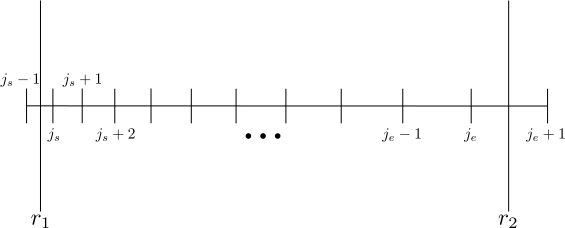
\includegraphics[width=0.95\textwidth]{globalcode_grid}
\caption[Radial grid used for discretizing linearized MHD
  equations]{Radial grid used for the discretization of the linearized
  MHD equations. There is one ghost zone outside of each boundary,
  which is used to specify the boundary conditions. The grid is
  equally spaced in $x=\ln{r}$.}
\label{fig:globalcode:globalcode_grid}
\end{figure}

The equations are evaluated with centered differences.  The quantity
$\beta_{r,j}$ indicates the value of $\beta_r$ at the $j$th
gridpoint. $\Delta x$ indicates the size of the grid step.

The following finite difference equations are found:
\begin{align}
\gamma\beta_{r, j} = &-(\frac{2\eta}{r_j^2 \Delta x^2} + \frac{\eta}{r_j^2}
 + \frac{\eta m^2}{r_j^2} + \eta k^2 + im\Omega_j )\beta_{r, j}
 + \frac{\eta}{r_j^2 \Delta x^2}(\beta_{r, j+1} + \beta_{r, j-1})
\nonumber \\
&- \frac{2im \eta}{r_j^2}\beta_{\theta,j} + k v_A \phi_{r,j}
\\
\nonumber \\
\gamma\beta_{\theta,j}=&-(\frac{2\eta}{r_j^2 \Delta x^2} 
 + \frac{\eta}{r_j^2} + \frac{\eta m^2}{r_j^2} 
 + \eta k^2 + im\Omega_j)\beta_{\theta, j}
 + \frac{\eta}{r_j^2 \Delta x^2}(\beta_{\theta, j+1} + \beta_{\theta, j-1})
\nonumber \\
&+\left[\frac{\Omega_{j+1}-\Omega_{j-1}}{2\Delta x}
 + \frac{2im\eta}{r_j^2}\right]\beta_{r,j} + kv_A\phi_{\theta,j}
\\
\nonumber \\
\gamma\phi_{r, j} = &-(\frac{2\nu}{r_j^2 \Delta x^2}
 + \frac{\nu}{r_j^2} + \frac{\nu m^2}{r_j^2} 
 + \nu k^2 + im\Omega_j)\phi_{r, j}
 + \frac{\nu}{r_j^2 \Delta x^2}(\phi_{r, j+1} + \phi_{r, j-1})
\nonumber \\
&+ \left[2\Omega_{j}-\frac{2im\nu}{r_j^2} \right]\phi_{\theta, j}
 - kv_A\beta_{r,j} - \frac{1}{2 r_j \Delta x}\left(\Pi_{j+1}-\Pi_{j-1}\right)
\\
\nonumber \\
\gamma\phi_{\theta, j} = &-(\frac{2\nu}{r_j^2 \Delta x^2} 
 + \frac{\nu}{r_j^2} + \frac{\nu m^2}{r_j^2} 
 + \nu k^2 + im\Omega_j)\phi_{\theta, j}
 + \frac{\nu}{r_j^2 \Delta x^2}(\phi_{\theta, j+1} + \phi_{\theta, j-1})
\nonumber \\
&+ \left[\frac{2im\nu}{r_j^2} - 2\Omega_j
 - \frac{1}{2\Delta x}\left(\Omega_{j+1}-\Omega_{j-1}\right)\right]\phi_{r,j}
 - kv_A \beta_{\theta, j} - \frac{im}{r_j}\Pi_{j}
\\
\nonumber \\
0 = &\left[\frac{2im\Omega_j}{r_j}
 + \frac{im}{r_j \Delta x}(\Omega_{j+1}-\Omega_{j-1})\right]\phi_{r,j}
 - \frac{2\Omega_j}{r_j}\phi_{\theta,j} 
\nonumber \\
&- \frac{1}{r_j \Delta x}\left(\Omega_{j+1}\phi_{\theta,j+1}
 -\Omega_{j-1}\phi_{\theta,j-1}\right)
 - \left[\frac{2}{r_j^2\Delta x^2} + \frac{m^2}{r_j^2}+k^2\right]\Pi_{j}
\nonumber \\
&+\frac{1}{r_j^2 \Delta x^2}\left(\Pi_{j+1} + \Pi_{j-1}\right)
\end{align}

\section{Boundary Conditions}

Boundary conditions are implemented by a set of constraint equations
at the inner and outer cylinders. The constraint equations are scaled
so that the terms in the equations are of the same order as the other
non-zero elements in the matrix.

\subsection{Velocity boundary conditions}

The hydrodynamic boundary conditions on $\phi_r$ and $\phi_\theta$ are
satisfied by $\phi_r = 0$ (no inflow) and $\phi_\theta = 0$ (no slip)
at the boundary.  There is a further no-slip constraint on $\phi_z$.
Because $\phi_z$ is not being solved for in the equations, this is
satisfied by setting $\partial_r^\dagger \phi_r = 0$ at the boundary,
implying $\phi_z=0$ by the incompressibility constraint. Since we have
already specified that $\phi_r=0$, this means that $\partial_r
\phi_r=0$ as well.

In the code, the constraints on $\phi_r$ are specified by setting the
values in the ghost zones
\begin{align}
\phi_{r,js-1} = 0, \quad \phi_{r, js} =& 0
\\
\phi_{r,je+1} = 0, \quad \phi_{r,je} = & 0
\\
\phi_{\theta,js-1} + \phi_{\theta,js}= &0 
\\
\phi_{\theta,je+1} + \phi_{\theta,je}= &0
\end{align}

\subsection{Magnetic boundary condition: perfectly conducting}

For this boundary condition, we consider the radial boundaries to be
perfectly conducting cylinders, rotating at a fixed speed. We make use
of the general boundary condition for a fluid with a moving interface$^3$
\begin{equation}
\hat{n}\times\left(\vec{E}_f - \vec{E}_c\right) = 
 \frac{\vec{v}\cdot\hat{n}}{c}\left(\vec{B}_f - \vec{B}_c\right) = 0
 \quad \text{for $\vec{v}\cdot\hat{n} = 0$.}
\end{equation}
where $\hat{n}$ is the unit vector normal to the conductor, pointing
into the fluid, and `$f$' and `$c$' indicate fluid and cylinder
values. Since the velocity at the boundary is purely azimuthal, where
the normal vector is radial, this states that the tangential component
of the electric field across the boundary is continuous.

For stationary conductors, the internal electric field is 0. But we
are considering a moving conductor, in which an electric field can be
generated to balance $\vec{v}\times\vec{B}$ in Ohm's law:
\begin{equation}
\vec{E} + \frac{1}{c}\vec{v}\times\vec{B}=\frac{4\pi\eta}{c^2}\vec{j}=0
\quad\text{for $\eta=0$.}
\end{equation}
We note that $\vec{v}=r\Omega\hat{\theta}$, and $\vec{B}=B_0\hat{z}$,
so the electric field in the conductor will be purely in the
$\hat{r}$-direction, and $\vec{E}\times\hat{n}=0$. So, we still find
that the tangential electric field is 0 at the boundary. To find the
implications of this on the magnetic field, we dot Faraday's law with
$\hat{n}$:
\begin{equation}
\left(\nabla\times\vec{E}\right)\cdot\hat{n} = 
-\frac{1}{c}\frac{\partial\vec{B}\cdot\hat{n}}{\partial t}
\end{equation}
The curl of $\vec{E}$ in the $\hat{n}$ comes purely from the
tangential components of $\vec{E}$, which we have shown are zero. We
find that $\partial B_r/\partial t = 0$, so $B_r$ is invariant in
time. Since out initial condition is $B_r=0$, we find $\beta_r=0$ at
the boundary.

To find the condition on $B_\theta$, we cross Ohm's law with $\hat{n}$:
\begin{equation}
\frac{4\pi\eta}{c^2}\vec{j}\times\hat{n} = \vec{E}\times\hat{n} +
 \frac{1}{c}\vec{v}\times\vec{B}\times\hat{n}=0
\end{equation}
Both terms on the right hand side are 0 at the boundary. We showed
previously that the tangential electric field, $\vec{E}\times\hat{n}$,
is zero. The $\vec{v}\times\vec{B}\times\hat{n}$ term is 0 because
$\vec{v}$ is purely azimuthal, and $B_r=0$, so $\vec{v}\times\vec{B}$
can only be in the radial (normal) direction. This means that there is
no tangential component of the current density,
$\vec{j}\times\hat{n}$, at the boundary. From Amp\`{e}re's law, this
implies that the tangential component of the curl of B is 0:
\begin{equation}
\left(\nabla\times\vec{B}\right)\times\hat{n} = 0
\end{equation}
Evaluating the axial component of the curl of $\vec{B}$, we see
\begin{equation}
\frac{1}{r}\frac{\partial}{\partial r}\left(r B_\theta \right)
 - \frac{1}{r}\frac{\partial B_r}{\partial \theta} = 0
\end{equation}
Since $B_r=0$ at the boundary, we find the boundary condition on
$B_\theta$, $\partial/\partial r (rB_\theta)= B_\theta +
r\partial/\partial r B_\theta = 0$.  Written in terms of our discretized
quantities and logarithmic coordinate $x$:
\begin{equation}
\beta_\theta + \frac{\partial}{\partial x}\beta_\theta = 0
\end{equation}

The values for the magnetic fields in the ghostzones are therefore
\begin{align}
\beta_{r, j_s-1} + \beta_{r, j_s} =& 0
\\
\beta_{r, j_e+1} + \beta_{r, j_e} =& 0
\\
\beta_{\theta, j_s-1} -
 \frac{(1 + 0.5\Delta x)}{(1 - 0.5\Delta x)}\beta_{\theta, j_s} =& 0
\\
\beta_{\theta, j_e+1} -
 \frac{(1 - 0.5\Delta x)}{(1 + 0.5\Delta x)}\beta_{\theta, j_e} =& 0
\end{align}

\subsection[Magnetic boundary condition: perfectly insulating]{Magnetic
boundary condition: perfectly
insulating\protect\footnote{Thanks to Jeremy Goodman for guidance in
implementing this boundary condition.}}

In the MHD approximation, Amp\`{e}re's law is
\begin{equation}
\nabla \times \vec{B} = \frac{4\pi}{c}\vec{j}
\end{equation}
In the insulating region outside the fluid, the current density is
zero, so the magnetic field can be written in terms of a scalar
potential
\begin{equation}
\vec{B} = \nabla\Phi
\end{equation}
Since $\nabla\cdot\vec{B} = 0$, we know that $\nabla^2 \Phi = 0$.  In
cylindrical coordinates, this means
\begin{equation}
\left[\frac{1}{r}\frac{\partial}{\partial r}r\frac{\partial}{\partial r} 
 + \frac{1}{r^2}\frac{\partial^2}{\partial\theta^2}
 + \frac{\partial^2}{\partial z^2}\right]\Phi = 0
\end{equation}
If we assume a form for $\Phi$ that goes as $\Phi(r,\theta,z) =
e^{i(m\theta + k z)}\tilde{\Phi}(r)$ this yields a differential
equation in $\tilde{\Phi}$
\begin{equation}
\frac{d^2}{d r^2}\tilde{\Phi} + \frac{1}{r}\frac{d}{dr}\tilde{\Phi} 
 - \left(\frac{m^2}{r^2} + k^2\right)\tilde{\Phi} = 0
\end{equation}
This equation is satisfied by modified Bessel fuctions
\begin{equation}
\tilde{\Phi}(r) = A_{in} I_m (k r) + A_{out} K_m (k r)
\end{equation}
Because $K_m(kr)\rightarrow \infty$ as $k r \rightarrow 0$ and
$I_m(kr) \rightarrow \infty$ as $k r \rightarrow \infty$, $A_{out} =
0$ in the inner region, and $A_{in} = 0$ in the outer region.
\begin{equation}
\tilde{\Phi}(r) = \begin{cases}
                     A_{in} I_m(k r), &r \le r_1 \\
                     A_{out} K_m(k r), &r \ge r_2
                  \end{cases}
\end{equation}
We evaluate $\nabla \Phi$ to find the components of the field
\begin{align}
B_r = &\frac{\partial \Phi}{\partial r} = e^{i(m\theta + kz)}
 \begin{cases}
   kA_{in}\left[I_{m+1}(kr) + \frac{m}{kr}I_{m}(kr)\right], &r \le r_1 \\
   kA_{out}\left[-K_{m+1}(kr) + \frac{m}{kr}K_{m}(kr)\right], &r \ge r_2
 \end{cases}
\\
\nonumber \\
B_\theta = &\frac{1}{r}\frac{\partial \Phi}{\partial \theta} 
         = \frac{im}{r}e^{i(m\theta + kz)}
           \begin{cases}
             A_{in} I_m(k r), &r \le r_1 \\
             A_{out} K_m(k r), &r \ge r_2
           \end{cases}
\end{align}

We now match the insulating solution to the magnetic field value just
inside the domain of interest to find $A_{in}$ and $A_{out}$. Once
those constants are known, the value of the magnetic field in the
ghost zone can be calculated. Note also the special case when $m=0$,
where $B_\theta$ at the boundary.

\begin{align}
\beta_{r, j_s-1} - \beta_{r, j_s}
 \frac{\left[I_{m+1}(kr_{j_s-1})+\frac{m}{kr_{j_s-1}}I_{m}(kr_{j_s-1})\right]}
      {\left[I_{m+1}(kr_{j_s})+\frac{m}{kr_{j_s}}I_{m}(kr_{j_s})\right]}
=& 0
\\
\beta_{r, j_e+1} - \beta_{r, j_e}
 \frac{\left[-K_{m+1}(kr_{j_e+1})+\frac{m}{kr_{j_e+1}}K_{m}(kr_{j_e+1})\right]}
      {\left[-K_{m+1}(kr_{j_e})+\frac{m}{kr_{j_e}}K_{m}(kr_{j_e})\right]}
=& 0
\end{align}
For $m \ne 0$:
\begin{align}
\beta_{\theta, j_s-1} - \beta_{\theta, j_s}\frac{r_{j_s}}{r_{j_s-1}}
 \frac{I_m(kr_{j_s-1})}{I_m(kr_{j_s})} =& 0
\\
\beta_{\theta, j_e+1} - \beta_{\theta, j_e}\frac{r_{j_e}}{r_{j_e+1}}
 \frac{K_m(kr_{j_e+1})}{K_m(kr_{j_e})} =& 0
\end{align}
For $m = 0$:
\begin{align}
\beta_{\theta, j_s-1} + \beta_{\theta, j_s} =& 0
\\
\beta_{\theta, j_e+1} + \beta_{\theta, j_e} =& 0
\end{align}

\section{Solving the equations}

The problem is to solve a system of $5N$ equations, where $N$ is the
number of gridcells including ghost zones. The equations can be cast
in the form of a generalized eigenvalue problem
\begin{equation}
{\bf A}\cdot{\bf x} = \gamma {\bf B}\cdot{\bf x}
\end{equation}
where $\gamma$ is the eigenvalue; ${\bf x}$ is the eigenvector made up
of the components $\beta_r$, $\beta_\theta$, $\phi_r$, $\phi_\theta$,
and $\Pi$ at each grid cell; ${\bf A}$ is a band-diagonal matrix of
bandwidth 15 that is made up of the terms in the linearized equations
and constraint equations; and ${\bf B}$ is a diagonal matrix with a 1
corresponding to the position of the evolution equation for each of
the quantities $\beta_r$, $\beta_\theta$, $\phi_r$, and $\phi_\theta$
in the fluid, and a 0 at the position of each boundary condition
equation and each constraint equation on $\Pi$.

Two methods are used to solve this generalized eigenvalue problem. The
first solves the full problem for all eigenvalues and
eigenvectors. Because resolutions of a few thousand grid cells are
sometimes necessary to fully resolve boundary layers, the calculation
of all the eigenvalues and eigenvectors can take a long time. A second
method can be used to solve for a subset of the eigenvalues and
eigenvectors, saving time in the calculation. In both cases the
eigenvalues and eigenvectors that are found are sorted are stored in a
\verb@NetCDF-4@ file for later analysis.

\subsection{Full solution}

The full solution method uses a call to the \verb@LAPACK@ routine
\verb@ZGGEV@
\footnote{Note about FORTRAN subroutine. Row-major versus column-major
  form, etc. Possibility of calls from Python, etc.}.  The routine
does not take advantage of the banded nature of the problem and takes
in $(5N)^2$ complex values describing the matrices ${\bf A}$ and ${\bf
  B}$, and requires additional memory allocation for its work. This is
not a very efficient mechanism, requiring large values of both time
and memory, as shown in Figure~\ref{fig:globalcode:timings}. On the
order of 20-30\% of the eigenvalues are spurious, with infinite
eigenvalues. These eigenvalues are rejected before saving the results.

\begin{figure}
\centering
\includegraphics[width=0.80\textwidth]{timings}
\caption[Execution time and memory scaling for global eigenvalue
  code]{Execution time and memory scaling for several different modes
  of operation of the global eigenvalue code. Solving the full problem
  for all eigenvalues becomes prohibitively difficult for large
  numbers of grid cells. Using the ARPACK subroutines results in
  dramatically more efficient operation, at the cost of increased
  complexity in setting up the problem.}
\label{fig:globalcode:timings}
\end{figure}

\subsection{Subset of eigenvalues}

The code has the option to use the \verb@ARPACK@ routine
\verb@ZNAUPD@. This routine supplies a reverse-communication interface
for the iterative technique, requesting calls to the \verb@BLAS@
routine \verb@ZGBMV@ and the \verb@LAPACK@ routine \verb@ZGBTRS@ to do
its work. Both of these routines can operate on compressed banded
matrices, requiring less memory than the method to generate the full
solution. \verb@ARPACK@ is a library that can be used to find a
number of extremal eigenvalues. This we are generally interested in
the largest growing modes, at first glance this seems to be a perfect
setup. Unfortunately, the \verb@ZNAUPD@ problem can only directly
solve for the largest growing modes if the matrix $B$ in the
eigenvalue problem is positive definite. In our case, it is positive
semi-definite (made up of `1's and `0's on the diagonal), and so we
are forced to use the routine in shift-invert mode, where a set of
eigenvalues $\lambda$ can be found that are related to the original
eigenvalues of the problem by $\lambda = 1/(\gamma-\sigma)$, where
$\sigma$ is a user-specified shift. This can be rewritten as
\begin{equation}
\lambda = \frac{\mathrm{Re}\{\gamma-\sigma\} - i\mathrm{Im\{\gamma-\sigma\}}}
               {|\gamma-\sigma|^2}
\end{equation}

The choice of $\sigma$, the eigenvalue shift, is very important for
correct behavior of the \verb@ARPACK@ routine, since it determines
which eigenvalues will be returned. To guarantee that we generate the
largest-growing eigenvalues $\gamma$, we would have to search for the
eigenvalues $\lambda$ of largest magnitude with $\sigma$ specified as
a very large real number. Unfortunately, as the value $\sigma$ gets
farther from the eigenvalues of interest, the routine becomes much
more efficient. So, $\sigma$ is chosen by an iterative technique.
$\sigma_0$ is initially chosen to be 5 times the inner cylinder speed
+ 5 times the outer cylinder speed, in order to assure that it will be
larger than the fastest growing mode, and the problem is solved with a
relatively large specified tolerance of $10^{-2}$. Next, a new value
of $\sigma_1$ is determined based on the largest-growing eigenvalue
$\gamma_0$, $\sigma_1 = 0.1\sigma_0 + 0.9\gamma_0$, and the
tolerance is halved. This process is repeated four times, and the
resulting $\sigma$ is then used to solve the problem at machine
tolerance.

While using the \verb@ARPACK@ subroutine results in greatly improved
performance, as shown in Figure~\ref{fig:globalcode:timings}, it comes
with some danger because of the importance of the choice of
$\sigma$. If it is chosen incorrectly, and is possible that some
eigenvalues of interest will be missed, or that spurious eigenvalues
will be generated, as is the case when $\sigma$ is almost exactly the
same value as one of the eigenvalues. Because of this, it is advisable
to verify some of the runs with the results from a full eigenvalue
calculation.

\section{Benchmarking}

\subsection{Narrow gap: Non-axisymmetric Alfv\'en waves}

This test case was run in a narrow gap with the inner cylinder at 20.2
cm, and the outer cylinder at 20.3 cm.  There was no background
azimuthal flow.  The applied field was 1000 Gauss, and $\eta$ and
$\nu$ were both 3.4e-3 cm$^2$/sec.  $k$ was 17.9 1/cm, and m was 1.
Several eigenmodes, with different effective values of $k_r$ are shown
in figure~\ref{fig:narrowgapalfveneigenmodes}.  The value of $k_r$ was
calculated for each mode, and the growth rate and oscillation
frequency are plotted again $k_r$ to yield the dispersion relation for
these modes.  The dispersion relation is plotted in
figure~\ref{fig:narrowgapalfven}.

\begin{figure}
\begin{center}
\includegraphics[width=0.80\textwidth]{narrowgap_alfven_eigenmodes.eps}
\caption{Alfv\'en eigenmodes with Pm=1 in a narrow gap. Modes with
  several different values of $k_r$ are shown.}
\label{fig:narrowgapalfveneigenmodes}
\end{center}
\end{figure}

\begin{figure}
\begin{center}
\includegraphics[width=0.80\textwidth]{narrowgap_alfven_pm1.0.eps}
\caption{Alfv\'en waves with Pm=1 in a narrow gap.  The lines indicate
  the analytic solution to the dispersion relation.}
\label{fig:narrowgapalfven}
\end{center}
\end{figure}

\subsection{Narrow gap: Non-axisymmetric Alfv\'en waves with Pm=0.1}

The same problem as in the previous section was repeated, but this
time with $\nu$ of 3.4e-3 cm$^2$/sec, to yield Pm=0.1.  In this case,
the modes stop oscillating at a sufficiently high $k_r$.  The
dispersion relation is plotted in
figure~\ref{fig:narrowgapalfvenpm0.1}.

\begin{figure}
\begin{center}
\includegraphics[width=0.80\textwidth]{narrowgap_alfven_pm0.1.eps}
\caption{Alfv\'en waves with Pm=0.1 in a narrow gap.  The lines
  indicate the analytic solution to the dispersion relation.}
\label{fig:narrowgapalfvenpm0.1}
\end{center}
\end{figure}

\subsection{Narrow gap: Non-axisymmetric inertial waves}
Inertial waves were examined in the narrow gap.  In this case, the
background flow rotated at a rate of 42 radians/sec, and there was no
background magnetic field.  $k_z$ was 1795 1/cm, and $\eta$ and $\nu$
were both 3.4e-3 cm$^2$/sec.  The dispersion relation for these modes
in shown in figure~\ref{fig:narrowgapinertial}.  The result again
matches the analytic dispersion relation.  The zero frequency modes in
this case correspond to zero-frequency alfven waves.  These waves are
completely decoupled from the inertial modes since $v_{A}=0$.

\begin{figure}
\begin{center}
\includegraphics[width=0.80\textwidth]{narrowgap_inertial.eps}
\caption{Inertial waves in a narrow gap.}
\label{fig:narrowgapinertial}
\end{center}
\end{figure}

\subsection{Axisymmetric MRI modes}

The code was used to solve the problem of the marginally unstable
eigenmode from the paper of Goodman and Ji with the following parameters
\begin{align*}
&\Omega_1 = 2720\,\mathrm{rpm} = 284.84\,\mathrm{rad/s},\quad
    &\nu = 3.2\times10^{-3}\,\mathrm{cm^2/s}
\\
&\Omega_2 = 328.4\,\mathrm{rpm} = 34.39\,\mathrm{rad/s},\quad
    &\eta = 2.0\times10^{3}\,\mathrm{cm^2/s}
\\
&r_1 = 5\,\mathrm{cm},\quad &\rho = 6.0\,\mathrm{g/cm^3}
\\
&r_2 = 15\,\mathrm{cm},\quad &B_0 = 3000\, \mathrm{gauss}
\\
&k = 2\pi n/h = 2\pi*0.5/10\,\mathrm{cm} = 0.314\,\mathrm{cm^{-1}}
\\
&N = 4000\,\mathrm{grid\,cells},\quad &\mathrm{Insulating\,boundaries}
\end{align*}

The spectrum of eigenvalues for the axisymmetric case, m=0, is shown
in figure~\ref{fig:goodmanm0eigenvalues}.  The unstable mode is shown
in figure~\ref{fig:goodmanm0unstablemode}.  This mode matches that
found in Goodman and Ji's paper.

The unstable mode has a $k_r$ such that a half-wavelength of the mode
spans the gap between the two cylinders.  The other, damped modes of
the system are modes with increasing $k_r$ as they are increasingly
damped.  A couple of typical eigenmodes, with two different values of
$k_r$, are shown in figure~\ref{fig:goodmanm0typicalmodes}.

\begin{figure}
\begin{center}
\includegraphics[width=0.80\textwidth]{goodman_m0_eigenvalues.eps}
\caption{Spectrum of eigenvalues for axisymmetric problem.  Eigenvalue
  with a slightly positive growth rate and zero frequency is the MRI
  mode.}
\label{fig:goodmanm0eigenvalues}
\end{center}
\end{figure}


\begin{figure}
\begin{center}
\includegraphics[width=0.80\textwidth]{goodman_m0_unstable_mode.eps}
\caption{Unstable MRI mode}
\label{fig:goodmanm0unstablemode}
\end{center}
\end{figure}

\begin{figure}
\begin{center}
\includegraphics[width=0.80\textwidth]{goodman_m0_typical_modes.eps}
\caption{Typical modes of the axisymmetric eigenvalue problem.  The
  modes span the gap with different values of $k_r$.}
\label{fig:goodmanm0typicalmodes}
\end{center}
\end{figure}

\subsection{Nonaxisymmetric modes}

Nonaxisymmetric modes of the MRI problem were also examined.  The
spectrum of eigenvalues for m=1 is shown in
figure~\ref{fig:goodmanm1eigenvalues}.  The nonaxisymmetric modes in
this case are all damped.  Typical eigenmodes of this problem are
shown in figure~\ref{fig:goodmanm1typicalmodes}.  The modes in this
case tend to be localized at some radius.  The oscillation frequency
of the mode is Doppler shifted by the fluid retation frequency at that
radius.  The shape of the velocity component of the modes is that of a
wavepacket.  But the magnetic modes often have tails that have a
finite value across the cylinder gap.

\begin{figure}
\begin{center}
\includegraphics[width=0.80\textwidth]{goodman_m1_eigenvalues.eps}
\caption{Spectrum of eigenvalues for nonaxisymmetric problem, m=1.}
\label{fig:goodmanm1eigenvalues}
\end{center}
\end{figure}

\begin{figure}
\begin{center}
\includegraphics[width=0.80\textwidth]{goodman_m1_typical_modes.eps}
\caption{Typical modes of the nonaxisymmetric eigenvalue problem.
  Each mode is localized near a specific radius.}
\label{fig:goodmanm1typicalmodes}
\end{center}
\end{figure}


\section{References}
1. M Nornberg, H. Ji, E. Schartman, A. Roach, and J. Goodman, Phys
Rev. Lett. {\bf 104}, 074501 (2010).

\noindent 2. J. Goodman and H. Ji, J. Fluid Mech. {\bf 462}, 365 (2002).

\noindent 3. T. H. Stix, {\emph Waves in Plasmas} (Springer-Verlag,
New York, 1992).
\end{document}
